\chapter{Application Deployment on AWS}
\section*{Introduction}
\addcontentsline{toc}{section}{Introduction}

Cloud deployment plays a crucial role in ensuring scalability,
availability, and reliability of modern applications. In this chapter,
we present the deployment strategy of our project on Amazon Web
Services (AWS). We describe the physical and logical architecture,
the containerization process, the deployment pipeline, and the
security measures implemented to protect the system.

\section{Project architecture}
\subsection{Physical architecture}
The physical architecture of our system consists of several interconnected layers, each serving a specific role within the overall project. Users interact with a mobile application developed in Expo, React Native, and TypeScript, providing a fluid and responsive interface for for service access.The system's core is a strong backend built with Node.js and TypeScript that manages user requests, business logic, and communication via a dedicated Python API.  A Chroma vector database, which contains all the necessary information for recommendations and optimizes user-specific suggestions, serves as the foundation for the recommendation system implemented by this Python API. Finally, all data is stored in a MongoDB database, , which guarantees the efficient and adaptable storage of user data and metadata required for the system to operate correctly.
\begin{center}
\begin{figure}[ht]
            \centering
            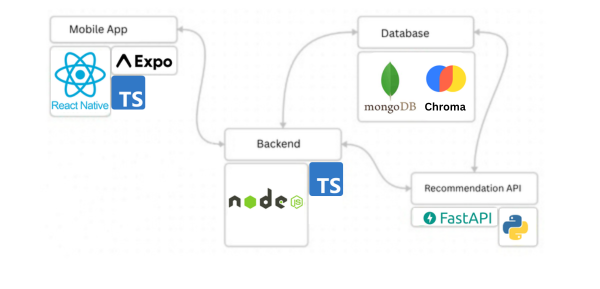
\includegraphics[scale=0.72]{images/physic_arch.png}
            \caption{Physical architecture of the system} 
            \label{fig:Physical architecture}
        \end{figure}
\end{center}
    
\subsection{Logical architecture}

\begin{center}
\begin{figure}[ht]
            \centering
            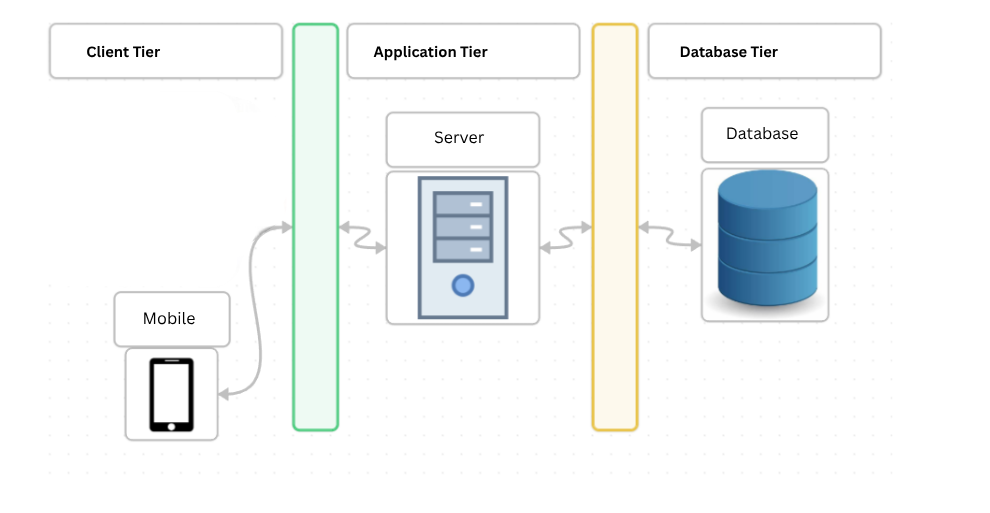
\includegraphics[scale=0.44]{images/logic_arch.png}
            \caption{Logical architecture }
            \label{fig:Logical architecture of the system}
\end{figure}
\end{center}


Our logical architecture of the system includes : a data layer, a middle layer, and a presentation layer.The data layer is responsible for information management and safe storage in an organized manner. Between the data layer and the presentation layer, the middle layer handles user requests, carries out business rules, and retrieves relevant data. The presentation layer consists of user interfaces accessible via a mobile application, enabling responsive and easy user interaction with the system.
This modular architecture enhences the scalability, maintainability, and flexibility of our application, which makes it ideal for future growth and or any adaptation.

\subsection{Containerization}
Containerization was achieved using \textbf{Docker}, which ensures
consistency across development, testing, and production
environments. Each component of the system was containerized:
\begin{itemize}
    \item \textbf{Backend (Node.js/TypeScript)} packaged as a
    container for handling API calls and business logic.
    \item \textbf{Python microservice} deployed separately to run the
    recommendation system using ChromaDB.
    \item \textbf{ChromaDB} persisted in a Docker volume to maintain
    vector embeddings.
    \item \textbf{MongoDB} containerized with persistent storage
    linked to an AWS EBS volume.
\end{itemize}

Containers communicate through a \texttt{docker-compose} network,
ensuring smooth orchestration and modular deployment.
\begin{center}
\begin{figure}[H]

\includegraphics[scale=0.23]{images/docker_compose.jpeg}
\caption{Docker compose logo}
\label{fig:docker_compose_logo}
\end{figure}
\end{center}


\subsection{Deployment}
The deployment is performed on \textbf{AWS EC2}, which acts as the
compute resource for hosting the application. The architecture
includes:
\begin{itemize}
    \item An \textbf{EC2 instance} running Docker and Docker Compose.
    \item An \textbf{attached EBS volume} of 20 GB (gp3) for persistent
    storage of ChromaDB and MongoDB data.
    \item \textbf{Nginx reverse proxy} configured as an entry point to
    route traffic to the FastAPI backend, with SSL certificates managed
    by Let’s Encrypt (Certbot).
    \item Security rules applied through \textbf{AWS Security Groups}
    (see next section).
\end{itemize}

This setup allows for scalability (via Auto Scaling Groups if needed)
and ensures data persistence with EBS volumes and automated
snapshots, as it is illustrated in the following figure.

\begin{center}
\begin{figure}[H]
\centering
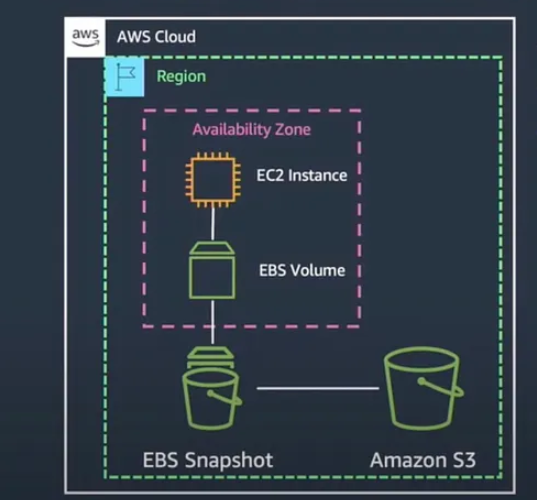
\includegraphics[scale=0.45]{images/AWS_architecture.png}
\caption{AWS architecture}
\label{fig:AWS_arch}
\end{figure}
\end{center}


\subsection{Security on Cloud}
Security is a critical aspect of cloud deployment. The following
measures were implemented:
\begin{itemize}
    \item \textbf{Security Groups:} firewall rules controlling traffic. Only
    ports 22 (SSH, restricted to admin IP), 80 (HTTP), and 443 (HTTPS)
    are open. Internal services (MongoDB, ChromaDB, FastAPI on port
    8000) remain private.
    \item \textbf{HTTPS encryption:} all traffic passes through Nginx with
    SSL/TLS enabled using Let’s Encrypt.
    \item \textbf{Data persistence:} MongoDB and ChromaDB volumes are
    stored on EBS, with daily automated snapshots for backup.
    \item \textbf{IAM roles:} AWS credentials for S3 backups and EC2
    management are restricted by least-privilege policies.
\end{itemize}

These measures ensure that the system is secure, reliable, and
compliant with industry best practices.

\newpage
\section{Deployment Challenges and Solutions}
During the deployment of the VitamiNurse application backend—comprising the recommendation system, AI assistant chatbot, and database on AWS—several significant challenges were encountered. These primarily concerned data persistence, backup strategies, and cost management.

\subsection{Ephemeral Storage Challenge}
A primary challenge stemmed from the ephemeral nature of the default storage on Amazon EC2 instances. An instance store provides temporary block-level storage that is physically attached to the host computer. Consequently, all data on this storage volume is irrevocably lost if an instance is stopped, terminated, or fails. This characteristic posed a severe risk to the integrity of the persistent ChromaDB vector embeddings and user data stored in MongoDB, rendering the default configuration unsuitable for a production environment.

\subsection{Storage solution: Persistent EBS Volumes}
The implemented solution was to attach an Amazon Elastic Block Store (EBS) volume to the EC2 instance as illustrated in Figure \ref{fig:ec2_ebs_persistence}. Unlike instance store volumes, EBS volumes provide persistent, block-level storage that exists independently from the life of an instance. By configuring the Docker containers to store the \texttt{./chroma\_db} data and MongoDB data on this attached EBS volume, the application's state is preserved across instance stops, restarts, or even instance migration.

\begin{center}
\begin{figure}[H]
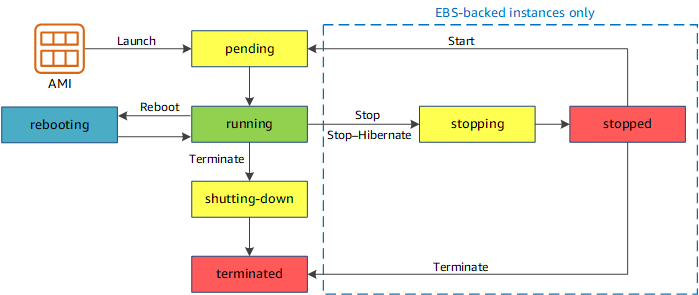
\includegraphics[scale=0.55]{images/ec2_instance_lifecycle.png}
\caption{EC2 lifecycle with persistent EBS volume for data retention.}
\label{fig:ec2_ebs_persistence}
\end{figure}
\end{center}
From a cost perspective, a 20 GB gp3 volume, which offers a baseline performance of 3,000 IOPS and 125 MB/s throughput, is priced at approximately \$0.08 per GB-month. This results in a monthly cost of \$1.60 for the primary persistent storage requirement.

\subsection{Data Backup and Recovery Challenge}
While an EBS volume ensures data persistence against instance lifecycle events, it does not inherently protect against data corruption, accidental deletion (e.g., via \texttt{rm -rf}), or the catastrophic failure of the Availability Zone. Relying solely on a single EBS volume constitutes a significant data loss risk.

\subsubsection{Recovery Solution: Automated EBS Snapshots}
To mitigate this risk, a strategy of automated EBS snapshots was implemented. EBS snapshots are incremental backups that are automatically saved to Amazon S3, providing a highly durable and reliable recovery point.

A common practice is to configure a daily snapshot schedule, which captures the state of the volume at 00:00 each day. The cost of EBS snapshots is based on the amount of data stored in S3, priced at approximately \$0.05 per GB-month. The initial full snapshot of a 20 GB volume would cost roughly \$1.00 per month. Subsequent incremental snapshots typically only store the changed data blocks. Assuming a daily change rate of 1 GB, the cost for incremental snapshot storage would be approximately \$0.05 per day, or \$1.50 per month. The total estimated cost for a robust daily backup strategy is therefore approximately \$2.50 per month.

\begin{center}
\begin{figure}[H]
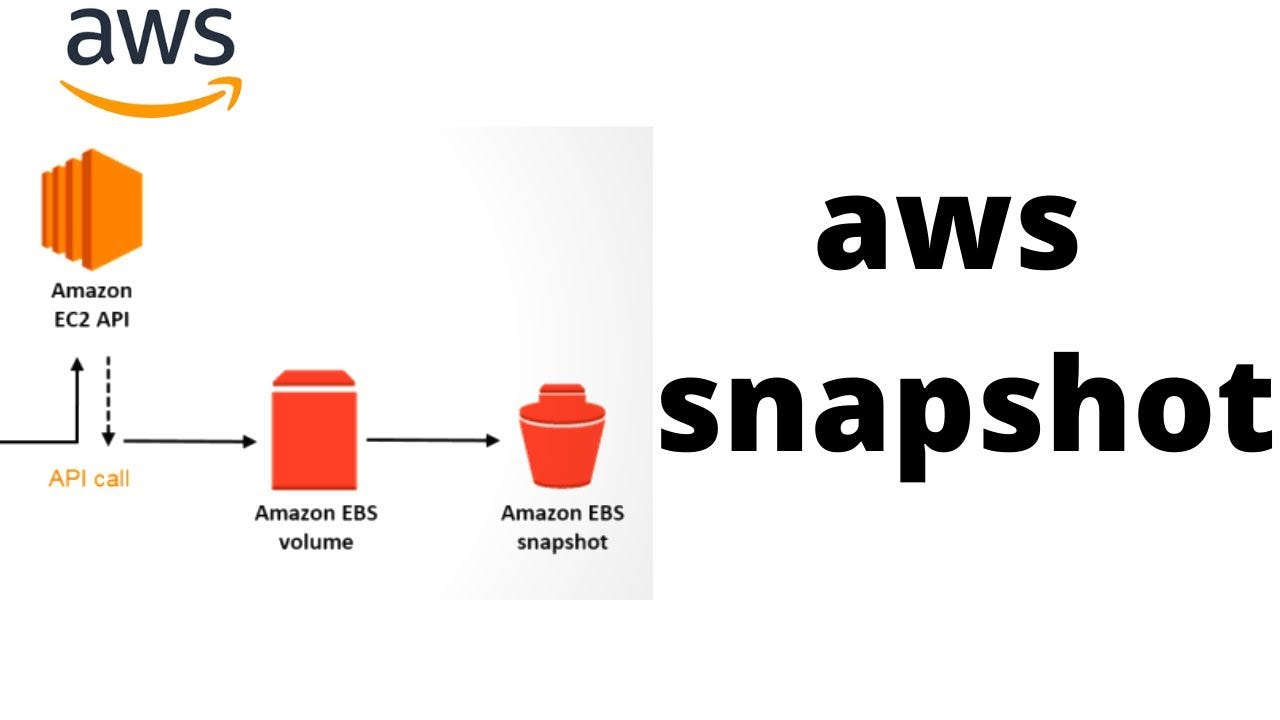
\includegraphics[scale=0.25]{images/snapshots.jpg}
\caption{Automated EBS snapshots}
\label{fig:snapshots}
\end{figure}
\end{center}

\subsection{Summary and Total Cost of Ownership}
The combined solution of a persistent EBS volume and automated snapshots provides a highly resilient and cost-effective storage architecture for the application. The ChromaDB and other critical data benefit from persistent storage, high performance, and automated, durable backups.

The total estimated monthly storage cost is calculated as follows:
\begin{itemize}
    \item EBS gp3 Volume (20 GB): \$1.60
    \item Automated Daily Snapshots: ~\$2.50
    \item \textbf{Total: ~\$4.10}
\end{itemize}

This architecture ensures that the application's data is not only persistent but also recoverable, aligning with production-grade reliability and disaster recovery best practices at a minimal cost.

\subsection{Next Steps: Deployment on Container Service}
While the EC2 deployment is functional, a more scalable and managed approach would involve migrating to a container orchestration service such as Amazon Elastic Container Service (ECS) or Amazon Elastic Kubernetes Service (EKS). These services abstract away the underlying EC2 instance management, automate container deployment and scaling, and integrate seamlessly with other AWS services like Application Load Balancers and AWS Fargate for serverless compute. This evolution would further enhance the application's scalability, resilience, and operational efficiency.

\section*{Conclusion}
In this chapter, we presented the deployment of our application on
AWS. We described both the physical and logical architectures, the
containerization of services using Docker, the deployment process on
EC2 with persistent EBS volumes, and the implemented security
strategies. Furthermore, we detailed the challenges of ephemeral storage and data backup, along with their cost-effective solutions. This deployment strategy ensures that our application is
scalable, cost-effective, and secure, making it suitable for real-world
use in production.